\documentclass[]{project_interim}
\bibliographystyle{apalike}
\bibstyle{apalike}
\usepackage{graphicx, wrapfig, listings}
\usepackage{hyperref}
\usepackage{cite}

\newcommand{\bulletPoint}{\hspace{-3.1pt}$\bullet$ \hspace{5pt}}

%---

\def\studentname{Dennis Marjanov}
\def\reportyear{2024}
\def\projecttitle{Human Computer Interaction}
\def\supervisorname{Susnas Sourjah}
\def\degree{BSc (Hons) in Computer Science (Software Engineering)}
\def\fullOrHalfUnit{CS3821 Full Unit}
\def\finalOrInterim{Interim Report}

%---

\begin{document}
\maketitle

%---

\chapter*{Declaration}
This plan has been prepared on the basis of my own work. Where other published
and unpublished source materials have been used, these have been acknowledged.
\vskip3em
Word Count:
\vskip3em
Student Name: \studentname
\vskip3em
Date of Submission: 13/12/2024
\vskip3em
Signature: Dennis Marjanov
\vskip0em


\newpage

%---

\tableofcontents\pdfbookmark[0]{Table of Contents}{toc}\newpage

%---

\begin{abstract}

  Human-computer interaction is at the core of how people engage with technology, forming
  a bridge between human intention and machine execution. This connection determines how
  effectively individuals can use computers and systems to accomplish tasks, from everyday
  things to life-critical processes. The design of these interactions must feel natural and intuitive, ensuring that users can easily understand and control complex technological systems.
  Effective HCI is key to minimizing human error, improving efficiency, and creating seamless
  experiences for all, from professionals to those less able
  \
\end{abstract}
\newpage

%---

\chapter{Introduction}
\section{Travel Planner}
Human-computer interaction is at the core of how people engage with technology, forming a bridge between human intention and machine execution. This connection determines how effectively individuals can use computers and systems to accomplish tasks. The overall aim for the project is to create interfaces which leverage HCI technique to create a better user experience.

The first interface will simplify travel planning as it is often a complex and time-consuming task, requiring users to commence research on many different areas such as weather, safety and costs. Existing tools such as AtlasObsucra overwhelm the user with a cluttered layout and heaps of information with little guidance on selecting the countries, rather only activities.

\begin{figure*}[ht!]
  \centering
  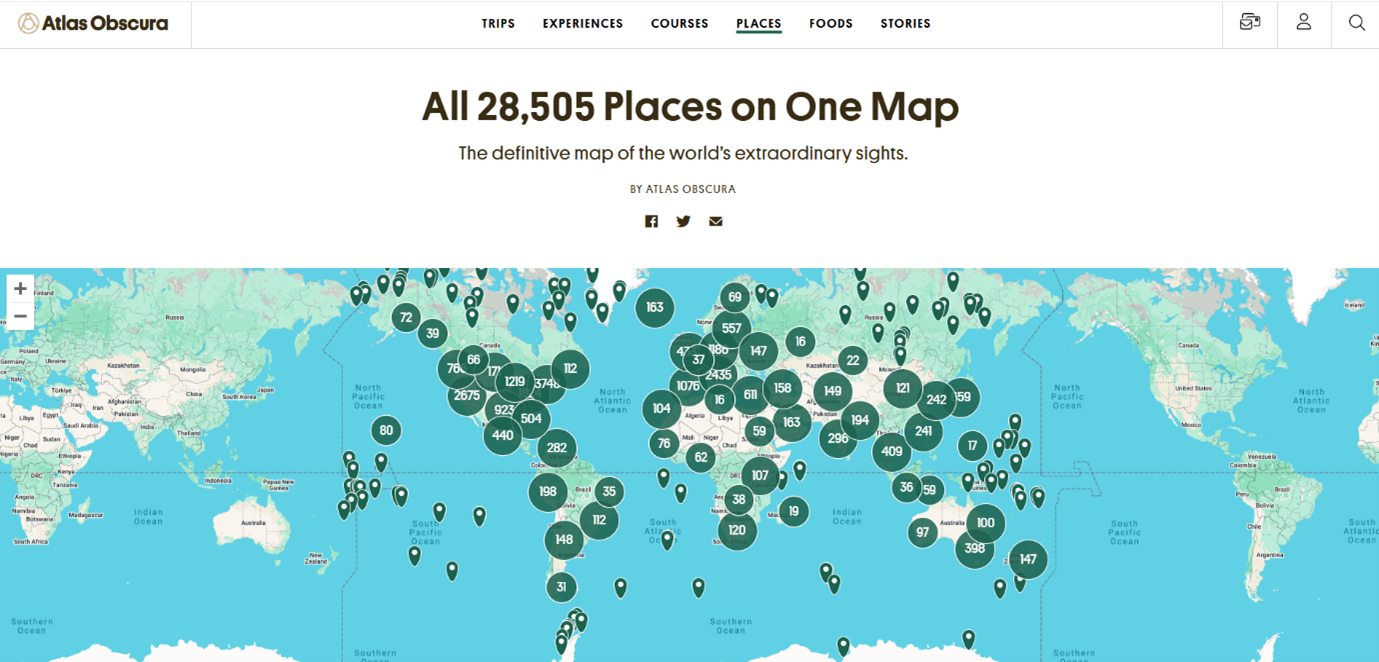
\includegraphics{atlasObscura.png}
  \vspace*{0.0cm}
  \caption{Atlas Obscura places exploration}
  \label{fig:1}
\end{figure*}

The image shows the method the website has chosen to display all of the places that you are able to visit, however circles showing things to do overlap, the same colour throughout doesn’t attract the user to any certain locations, and there is no way for the user to get a gist of the place or important information with ease from the website. All of this is poor human computer interaction and will increase the cognitive load of the user due to the number of options available and lack of guiding across the website.
Another popular example is called lonely planet. The website offered guides and information on all travel destinations around the world. However the format that it is presented restricts or bores the user.

\newpage

\begin{figure*}[ht!]
  \centering
  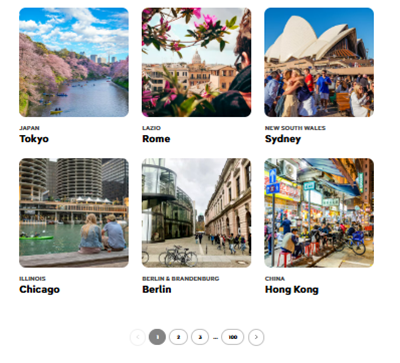
\includegraphics{lonleyPlanet.png}
  \vspace*{0.0cm}
  \caption{Lonely Planet exploration page}
  \label{fig:1}
\end{figure*}

A grid of 12 cities per page with over 100 pages to explore would cause the user mental fatigue and there is a high probability that they would not go through all the designations due to the format that they are presented. Therefore, the website has not done a good job at presenting the information and options in the world. As well as lacking intuition or guidance for the user to use their natural human urge for exploration.

An aim of simplifying Travel planning to use intuition and reducing cognitive load forces us to use recognisable formats such as an interactive 3d globe and creates many objectives. These include to create a 3D globe that is interactive, displaying visual data using intuitive colour coded gradients, for example regarding temperature, red for warmer regions while blue will be for cooler regions. The visual data will change depending on the selected month in the menu and instantly update the globe to reflect the data selected. These aims have been created to make data interpretation easier as well as reducing cognitive load by associating specific data to colours.

\newpage

\section{Recipe App}
The second interface was created to tackle common challenges elderly people and visually impaired users will face with cooking apps, such as cluttered layouts, small text and interfaces that require multiple actions that are unnatural to humans.

The Cremes app is a cooking app which I found to be one of the best in the market currently in regard to human computer interaction. However it is not very inclusive, with a dark background and colour scheme which is fixed, some users may struggle to see the buttons which provide options. Multiple options in navigation from being able to swipe down and see multiple different categories as well swiping to the side to view recipes within those categories is too complex for elderly users that haven’t grown up with phones. Furthermore, some concepts may be unfamiliar to users who haven’t had experience with social media, such as the concept of posting stories.



\begin{figure*}[ht!]
  \centering
  \begin{minipage}[t]{0.4\textwidth}
    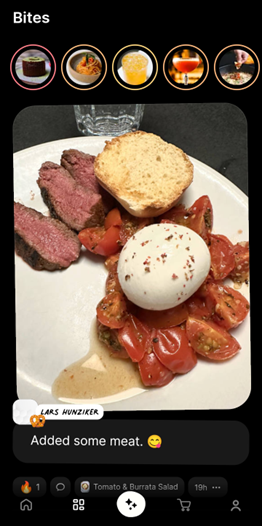
\includegraphics[width=20em]{cremeImage1.png}
  \end{minipage}
  \hfill
  \begin{minipage}[t]{0.4\textwidth}
    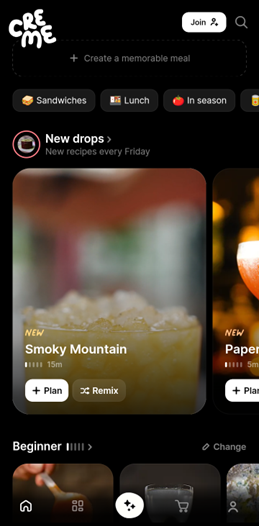
\includegraphics[width=20em]{cremeImage2.png}
  \end{minipage}
  \caption{Creme HomePage and recipe page}
  \label{fig:1}
\end{figure*}

With the sleek but packed interface cognitive load will not be reduced for the user which is negative as the aim is for the user experience to be as smooth and seamless as possible.
To improve I will be Aiming to enhance accessibility in cooking for elderly and visually impaired users through simplified navigation and a high contrast or custom palette design. Creating the objectives of designing a user-friendly login screen with large, high contrast text and customisable font sizes and colour schemes, giving the user options to enhance their experience. Next, I will implement a prototype for the recipe selection interface ensuring a clear layout, as well as simplify navigation by focusing on one instruction per page for clarity and usability.

A further issue with this app is its lack of clarity when it comes to starting the recipe, instead of following simple and coherent terminology such as start or begin they have chosen to use the word plan amongst the layout, this doesn’t stand out to the user and indicate an immediate call to action to them.

\begin{figure*}[ht!]
  \centering
  \begin{minipage}[t]{0.4\textwidth}
    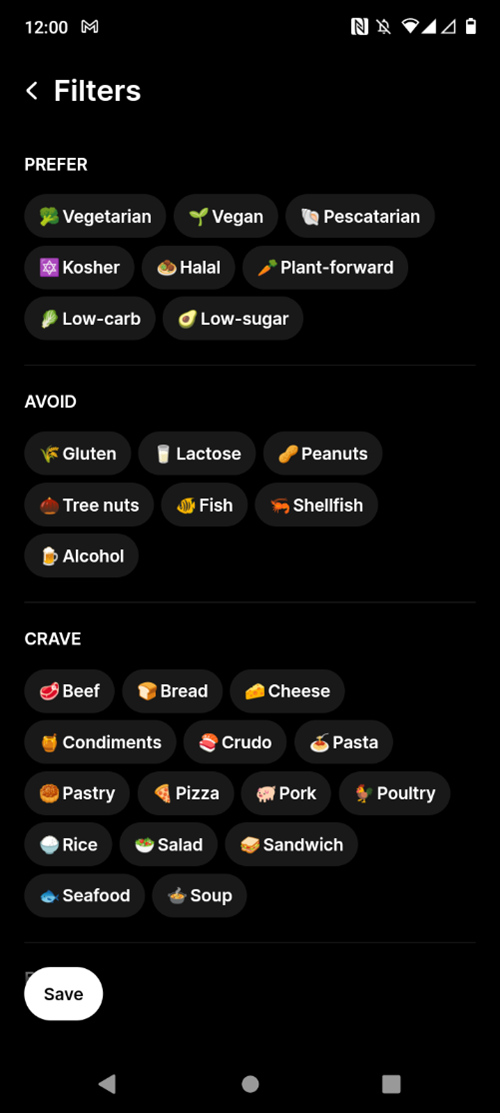
\includegraphics[width=20em]{cremeImage3.png}
  \end{minipage}
  \hfill
  \begin{minipage}[t]{0.4\textwidth}
    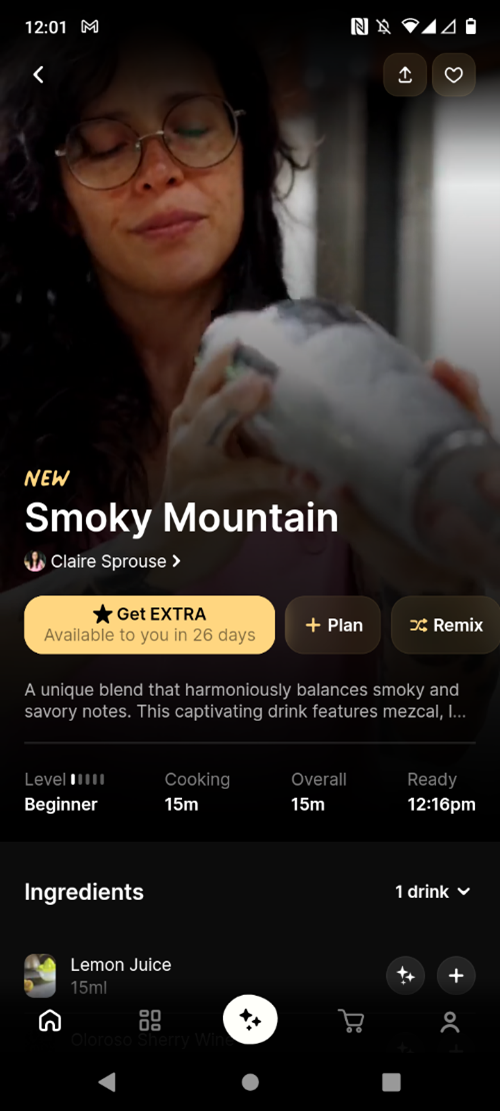
\includegraphics[width=20em]{cremeImage4.png}
  \end{minipage}
  \caption{Creme filters and selected recipe page}
  \label{fig:1}
\end{figure*}

Aspect of the application I did like was the user of icons throughout next to the text, this gives the user multiple forms of feedback on the screen. The consistency throughout the app is also something that I will be aiming for however with simplified interactions, and a better flow through the application inhibiting the user to wander off away from the task, which is: to select a recipe and follow it.

\section{Art Gallery}

The third interface identified a problem with the Online Art gallery Market, many platforms focus on transactions for business but neglect the user experience and the artists expression and presentation. Existing system often lack engaging visuals or clear navigation paths that would encourage exploration of different art.
Throughout research it seems that there is a common theme throughout the art galleries, all of the art shown is in grids with white backgrounds, and all of the artists pages are plain and simple with text and their work. This could be improved by connecting the user and the artist through their page, if the artist uses a certain colour palette, I will use that palette for the artist’s page. Different fonts could represent different people, clear and concise fonts would be a good depiction for architectural art while gothic or less coherent fonts would be suitable for abstract artists.

\begin{figure*}[ht!]
  \centering
  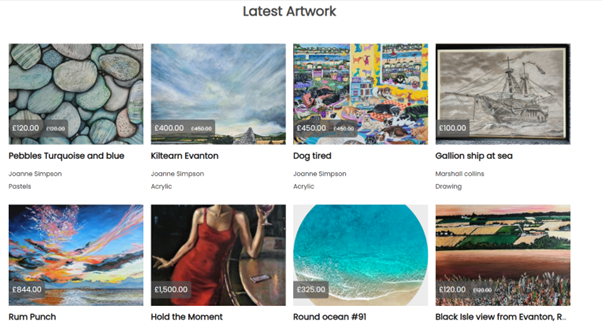
\includegraphics{artGalleryGrid.png}
  \vspace*{0.0cm}
  \caption{Example of online Gallery layout}
  \label{fig:1}
\end{figure*}

\newpage

Artsy is one of the largest online selling platforms of art in the world with a lot of information and content. To improve firstly we would need to simplify the website to show just necessary information and through progressive disclosure more can be revealed as per the users requests.
The next alteration I will make it creating the website more personal to the user and the page to represent the artist. Examples of good design for the user and artist have been shown below:

\begin{figure*}[ht!]
  \centering
  \begin{minipage}[t]{0.4\textwidth}
    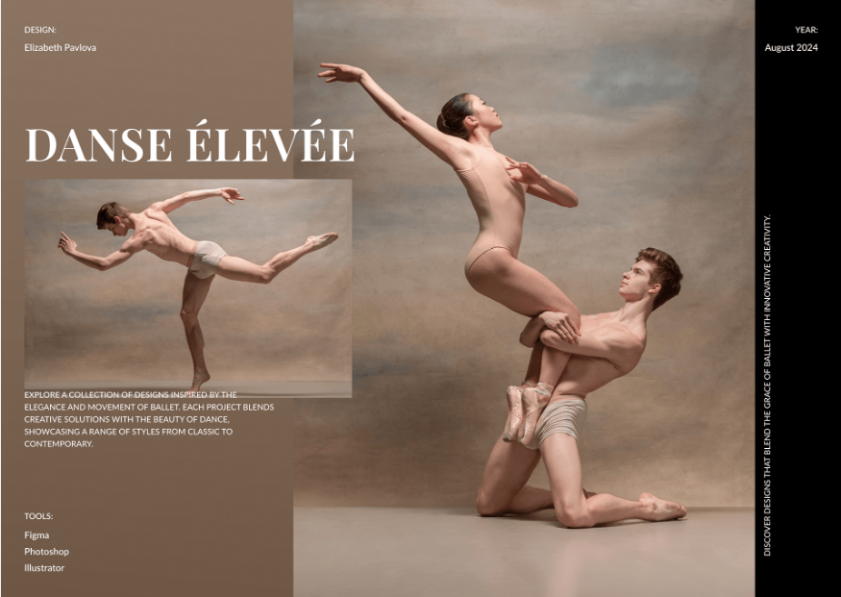
\includegraphics[width=20em]{artGalleryExample.png}
  \end{minipage}
  \hfill
  \begin{minipage}[t]{0.4\textwidth}
    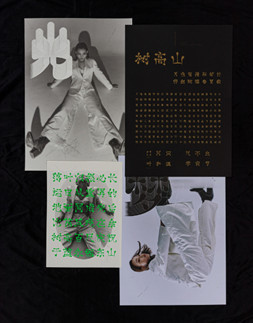
\includegraphics[width=20em]{artGalleryExample2.png}
  \end{minipage}
  \caption{Example of good layouts to showcase artists}
  \label{fig:1}
\end{figure*}


\chapter{Planning and Time Scale}
\section{Milestones and Reflection}
The Travel Planner has met all of the requirement’s set out for the early deliverables. The basic functionality of the globe has been implemented and data is visually mapped onto the globe in a colour gradient depending on the filters selected and month.
This foundation will set me up for the final deliverables as the code for mapping data and colours has been created and I better understand how to use layers on the globe to reach the desired functionalities.
Further code has been created in regards to the Travel Planner which has not been implemented such as code which recognises the country that the user selects, meaning that development of selection of countries and opening new pages of off the event will be easier.

The Recipe App with one instruction per page has also met all of the necessary milestones and target to be able to meet the final deliverables. The foundations of the app have been set in forms of the majority of the navigations developed as well as the more complex areas of code which will change the font size and colour palettes of the app for the users’ needs and desires.

My term 1 timeline provided realistic goals and achievable weekly targets which meant that a substantial amount of progress was made. The iterative approach of incorporating feedback at multiple stages reduced the risk of big weaknesses within the development and deliverables. However it did not account for large delays or technical challenges which should have been expected due to new technologies used.

The term 2 timeline will now have more time for anticipated delays and testing will be implemented to receive feedback on the interfaces and make any changes before the deadline. Complex features such as the Travel Planner will be prioritised at the start to ensure that they are developed and finished. The same will be done for the recipe app and advanced features.

A testing phase will be implemented near the end of the timeline and include user testing.



\section{Term 2}

\scalebox{1}{
  \begin{tabular}{r |@{\bulletPoint} l}
    Week 1 - 2  & Add more datasets, make countries interactable and add more information   \\
    Week 3 - 4  & Develop itinerary generation and finalize travel planner.                 \\
    Week 5 - 6  & Act on supervisor feedback, change structure, add images                  \\
    Week 7 - 8  & Develop interface based on wireframes                                     \\
    Week 9 - 10 & Test all projects, have others test and provide feedback, act on feedback \\
    Week 11     & Submit final deliverables and project report.                             \\
  \end{tabular}
}

%---

\chapter{Theory}
\section{Cognitive Load}
Sweller developed the cognitive load theory during while researching how "instruction design interacts with the cognitive architecture of human memory". The goal of cognitive load theory is to optimize learning by managing the mental effort required to process information. There are 3 components to the theory, long term memory, working memory and schema. The working memory is responsible for the processing of information via either the visuospatial subsystem which process visual and spatial information such as images and written text. The other method is through the phonological subsystem which handles auditory and verbal information such as speech. This theory directly relates with the design and layout of online interfaces as the interfaces directly interact with the users working memory, if the interface is poorly designed the working memory can be overloaded which would lead to frustration, errors and abandonment by the user.

The theory identifies 3 types of cognitive load including intrinsic, extraneous and germane load which all effect the user in different ways and have different methods of minimisation.\cite{de_jong_cognitive_2010}\cite{schnotz_reconsideration_2007}

\subsection{Intrinsic Load}

Intrinsic load is caused by the inherent complexity of the tasks that the users must perform or the information that they must process on an interface. The load depends on the level of interactivity which refers to the extent to which the user will understand the task. Tasks with high interactivity are complex while tasks with low interactivity are simpler. However the level of interactivity is dependant on the user and their past experiences which are stored in the schema. For example, you had to translate a sentence from English to Spanish, the task will be high interactivity for users that do not speak Spanish, however low interactivity for users who speak both languages.

This has a big impact on the users as high intrinsic load can overwhelm the users which leads to frustration and a higher percentage of errors. Or worst the user could not engage with the tasks at hand and leave the interface. This is poor HCI as the aim is always to keep the user engaged.

To ensure that intrinsic load does not cause negative impacts on the users there are many methods to lower the load, for example breaking down the information of a larger task into smaller and simpler steps for the user to follow. Another method would be to provide the user with tools to guide them through certain tasks, such as templates or extra information. Progressive learning is also a technique which is recommended and directly related to online interfaces in my project. This is because progressive learning refers to isolating simpler elements before showing the full complex task. For example, a filter button may hide a modal screen with many filters available, but they are hidden behind the button to reduce the intrinsic load for the user.\cite{sweller_element_2010}

\subsection{Extraneous Load}

Extraneous load refers to the cognitive effort caused by poorly designed interfaces and is directly related to how the information is presented to the user. Cluttered layouts would overwhelm the user with too much information displayed poorly for the working memory to understand. Furthermore redundant content could force users to process unnecessary data increasing the load.

Increased extraneous load increases the users mental effort without helping towards the task completion and can frustrate users which causes a higher percentage of errors to be made during the tasks.

To reduce the extraneous load the design of the interface should be simplified , clean and uncluttered, this means that any data or information that is obsolete or not needed should be removed as well as duplicated. Another way to reduce would be to follow common design principles for interfaces such as visual hierarchy and Gestalt principles to guide the users attention correctly.\cite{todorovic_gestalt_2008}\cite{moller_what_2012}

\subsection{Germane Load}

Germane Load refers to the mental effort needed for learning and understanding and developing our schema. This is considered a positive load and we want to be able to increase it to the maximum without effecting the intrinsic or extraneous load. It is crucial in how interfaces are structured as the load helps recognise patterns, apply concepts and learn new information without any prior knowledge. This is because it focuses on active learning and pattern recognition and is stimulated by tasks such as connection past experiences to new information which highlights why interfaces must be kept consistent throughout as the user is constantly learning how to interact with it and recognising patterns.

The Germane load is increased when the user is included in interactions such as tutorials or challenges. Prompts to engage the user or focus attention would be equally as effective. Another effective strategy is to reinforce patterns by using consistent layouts and symbols to enforce learning and interaction as the user becomes more comfortable on the interface.

\subsection{Progressive Disclosure}

Progressive Disclosure is a principle that reveals information gradually to the users, reducing cognitive load and allowing users to focus on only the current task as they do not have access to further ones. As mentioned before the Travel Planner incorporates this theory within the filters as the individual filters are hidden behind a dropdown menu. The menu which hides the filters at first reduces complexity. This approach in design on the interface aligns with the findings from the Interaction Design Foundation which has stated that progressive disclosure improves usability. However this approach has also been used on the Recipe App as the instructions are presented sequentially, this will simplify the navigation. Each page contains enough information to complete a small task from a larger set of decomposed tasks to make the recipe.\cite{noauthor_progressive_nodate}

\section{Visual hierarchy and eye tracking}

Visual Hierarchy and eye tracking are concepts that are user in the interface to create a better user experience. Together they explain how users interact with visual content and navigate interfaces through studies which track the human eyes natural behaviour when interacting with a interface. Understanding the principles of visual hierarchy and the eye tracking studies will lead more efficient interfaces which better cater to the users needs.\cite{wang_eye-tracking_2014}

Visual Hierarchy refers to the arrangement of elements on the page to guide the user in a structured manor. This means that the user will be directed to the most important information first as well as understand relationship or connected content and components in the interface.\cite{noauthor_what_nodate}\cite{noauthor_visual_nodate}

According to Djamasbi, visual hierarchy determinds the sequence in which the user will process content on the screen. Effective Hierarchy focuses attention and reduces cognitive load. The sequence can be impacted by many different principles such as:

Size - Larger elemenets on the interface will attract more attention as demonstrated by Faraday who conducting an experiement on directing search behaviour with size.

Contrast - High contrast between elements makes the content easier to read and understand.

Colour - Vibrant or bold colours enmphasis specific elements while muted tones will go into the background.

Positioning - Lavie and Tractinsky showed that central placement often correleates with user engagement due to a natural gaze pattern from user behaviour.
\cite{djamasbi_eye_2014}\cite{djamasbi_generation_2010}

Eye tracking is the measurement of eye movement to understand how users will interact with interfaces. It shows the natural flow of user attention and identifies which part of the interface capture the most attention. This can help with optimising the layout of an interface to improve usability and the user experience. The Nielsen Norman Group found that users follow similar predicatble patterns such as the F-pattern or the Z-pattern which were found via heatmaps which reveal "hot zones" where attention is concentrated such as the central and upper left areas of the page.



\section{Colour Theory}

Colour theory is the study of how colours interact and effect both human emotions , perceptions and behaviours. The relationship between colours can be manipulated to convey information or make the user feel a certain type of way. This is important to the interface as designs and colours can bring attention to certain information and build trust between the user and the interface.
Furthermore, colours have an emotional impact as they can evoke feelings and influence how the users perceive the information or interface that they are interacting with. This also leads into accessibility as colours can help ensure that the content on the interface is usable for individuals with visual impairments such as colour blindness.\cite{cyr_colour_2010}

Colours have physchological effects and can evoke subconcious responses, for example:

Red = Urgency or danger and is used for notifications or warnings
Blue = Trust, calmness, relaiability and is used in healthcare designs in hospitals
Green = Saftey, heatlh and is also used is hospitals
Yellow = Energy , attention
Black = Power, simplicity and is often used in luxury brands
White = Purity, cleanliness and promotes simplicity

Faraday found that bright colours such as red or yellow attrack the users attention more than others  which is why call to action buttons often use bright colours to navigate the users actions. The study showed that the colours were attention grabbing due to their high visability and cultural associastions such as warning signs.

Lynch and Horton provided research which shows the effects of inconsistent or improper colour use which cause cognitive challenges including visual fatigue and user frustration. Consistency in colour application reduces cognitive strain.
This means that buttons such as home or back should have the same throughout the interface to avoid disturbing the user flow.\cite{fialkowski_considering_2024}

Meyer looked into cultural influences on colour interpretation and showed how culture plays a significant role in the perception of colours. For example western cultures see the colour Blue for trust and professionalism, as shown by its use in the healthcare system.
However eastern cultures symbolise colours such as Red for good fortue or celebration or white for mourning.
This means that interfaces can be further imporved if the colours used matched the culture the interface is used in.


\section{Accessibility design}

Accessibility in design refers to the practise of creating interfaces that are usable by everyone regardless of their abilities or disabilities. This means that during the design we will need to consider a variety of different users and the struggles that they might face from auditory, visual , cognitive challenges for example.
Standards such as the Web Content Accessibilit Guidelines (WCAG) provide frameworks for achieving accessible designs for all users by following certain prinicples.\cite{initiative_wai_wcag_nodate}

Achieving an accessible design is important in the interface as it ensures equal access of technology for all users as well as being a legal requirement in many countries. The UK has an eqality act while America has a law called Americans with Disabilities (ADA). Damage could be done to companies and interfaces if the law is not followed as governing bodies have the power to impose penalites as well as cause reputational damage.
Interfaces would also have interest in designing for accessibility as they will now be available to a much larger audience as it is estimated that 15 percent of the global population have some sort of disability.

Nielsen stated that accessibility improves the usability of the interface for all users not just users with impairments and created a concept called "Universal design".
This refers to simplifying navigational structures to benefit users with cognitive disabilities and first time users at the same time. For example the recipe app with one instruction per page will reduce cognitive load for the elderly users however the navigation will be simpler for all users now.\cite{noauthor_accessibility_nodate}

Meyer and Rose proposed that learning envirnments and tools should be available to accommodate for many different learning styles and abilities. Meaning customisable settings for font size, contrast and colours to cater to users with visual impairments. This would impact a lot of potential users according to the World Heatlh Organisation (WHO) who found out the approximately 2.2 billion people have a visually impairment globally. This shows the need for accessibility design.\cite{noauthor_world_nodate}

\chapter{Project Description}
\section{Travel Planner}

The Travel Planner is an interactive web application that has been created with the aim of simplifying the process of exploring Travel desintations around the world. It provides essential travel data to the user - temperature, rainfall and safety- on a 3d globe which is interactive. Using concepts such as visual hierarchy and cognitive reduction techqunices the data is mapped onto the globe visual through intuitive colours as an alternate to text based information currently.

The aim of creating a travel planner by focusing on visualising complex data for all users to understand many objectives for the early deliverables arised.
Firstly I needed to create a 3d globe that the users would be familiar with and have the ability to interact with through a variety of actions. On this globe colour gradients would represent data that is being presented, the colours chosen needed to be intuitive and universatlly understandable by the users, for example warm colours where used to present data of hotter counties in some months.
Furthermore, the interface needed filters for month specific data as holidays and travel on average last 8-10 days within a month. Therefore showing broad yearly data would not be relevant. Once a month is selected the user should have freedom to view different datasets by selecting different information the are interested in, for example , rainfall that month, temperature or safety of the county.
Saftey of countries changes by month as well, for example in brazil, Feburary would be a dangerous month in 2024 due to carnival falling inside the month, meaning crime rates are higher and with an increase of tourists so does the petty crime.

\subsection{Relation to HCI}

The Travel Planner is an interactive web application that has been created with the aim of simplifying the process of exploring Travel desintations around the world. It provides essential travel data to the user - temperature, rainfall and safety- on a 3d globe which is interactive. Using concepts such as visual hierarchy and cognitive reduction techqunices the data is mapped onto the globe visual through intuitive colours as an alternate to text based information currently.

The aim of creating a travel planner by focusing on visualising complex data for all users to understand many objectives for the early deliverables arised.
Firstly I needed to create a 3d globe that the users would be familiar with and have the ability to interact with through a variety of actions.

\begin{figure*}[ht!]
  \centering
  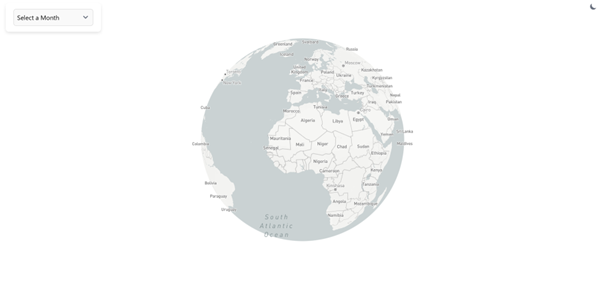
\includegraphics[width=\textwidth]{TP-plain.png}
  \vspace*{0.0cm}
  \caption{Recipe App Class Diagram}
  \label{fig:1}
\end{figure*}

\newpage

On this globe colour gradients would represent data that is being presented, the colours chosen needed to be intuitive and universatlly understandable by the users, for example warm colours where used to present data of hotter counties in some months.

\begin{figure*}[ht!]
  \centering
  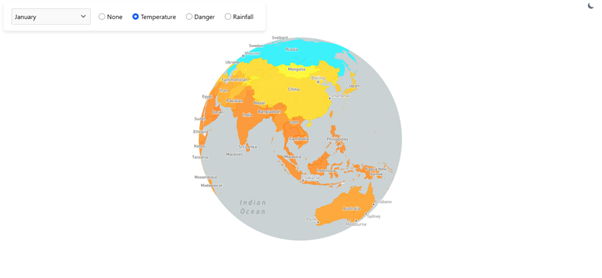
\includegraphics[width=\textwidth]{TP-Temp.png}
  \vspace*{0.0cm}
  \caption{Recipe App Class Diagram}
  \label{fig:1}
\end{figure*}

Furthermore, the interface needed filters for month specific data as holidays and travel on average last 8-10 days within a month. Therefore showing broad yearly data would not be relevant. Once a month is selected the user should have freedom to view different datasets by selecting different information the are interested in, for example , rainfall that month, temperature or safety of the county.
Saftey of countries changes by month as well, for example in brazil, Feburary would be a dangerous month in 2024 due to carnival falling inside the month, meaning crime rates are higher and with an increase of tourists so does the petty crime.

\begin{figure*}[ht!]
  \centering
  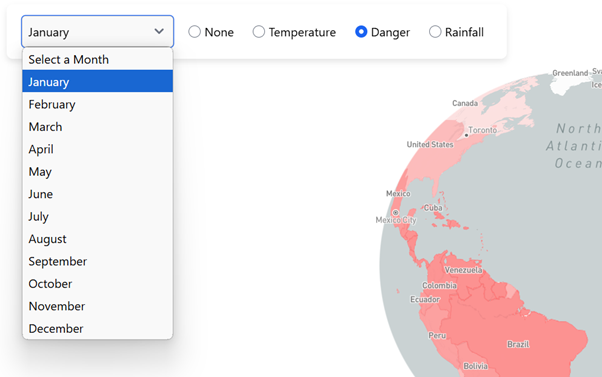
\includegraphics[width=\textwidth]{TP-nav.png}
  \vspace*{0.0cm}
  \caption{Recipe App Class Diagram}
  \label{fig:1}
\end{figure*}

The travel planner reduces extraneous load by using techniques such as progressive disclousure through dropdown menus that hide complex filters or multiple options to the user. This aligns with swellers research and the finding which show that reducing unnecessary cognitive load increases learning and interaction within interfaces.
Germane load is also supported through the consistent use of colour throughout, this will help users recognise patterns such as warm colours represent higher temperatures and cool colours represent lower temperatures.

Eye Tracking studies have showed us that visual hierarchy is important in what the users sees first on the interface. The placement of the 3d globe uses central fixation bias (djamasbi) which ensures that the users attention is drawn to the most important element on the screen (3d globe). Visual elements such as drop down menus are placed in close promximity to the globe showing the user that their is a relation between the 2 elements. This follows Gestalts principles of proximity and alignment\cite{todorovic_gestalt_2008}.

In regaurds to accessibility the interface includes an intuitive navigation cia a simple drag or zoom control which the majority of users are familiar with due to past experiences and developed schema. These controls align with the Web Content Accessibility Guidelines (WCAG) and their principles of perceivability and operability.\cite{initiative_wai_wcag_nodate}



\section{Recipe App}

The Recipe app is an android based application that simplified cooking for elderly and visually impaired users by presenting one instruction per page. To cater for target users I have implemented features such as customisable text sizes and colour palettes to ensure inclusivity.
The aim of enhancing the accessibility of online cooking apps meant that I need to offer customisable settings and tools to include a larger variety of users. Use one instruction per page to reduce cognitive load and implement intuitive navigation throughout the application.

\subsection{Relation to HCI}

Accessibility is the main focus of the application meaning that the interface follows perceivabilioty by offering high contrast colour schemes as one of the options and operability through large tappable buttons, addressing the needs to the user. The customisable font size and colour pallettes align with the WCAG principles which ensure that all of the users are able to tailor the application to their needs.

\begin{figure*}[ht!]
  \centering
  \begin{minipage}[t]{0.4\textwidth}
    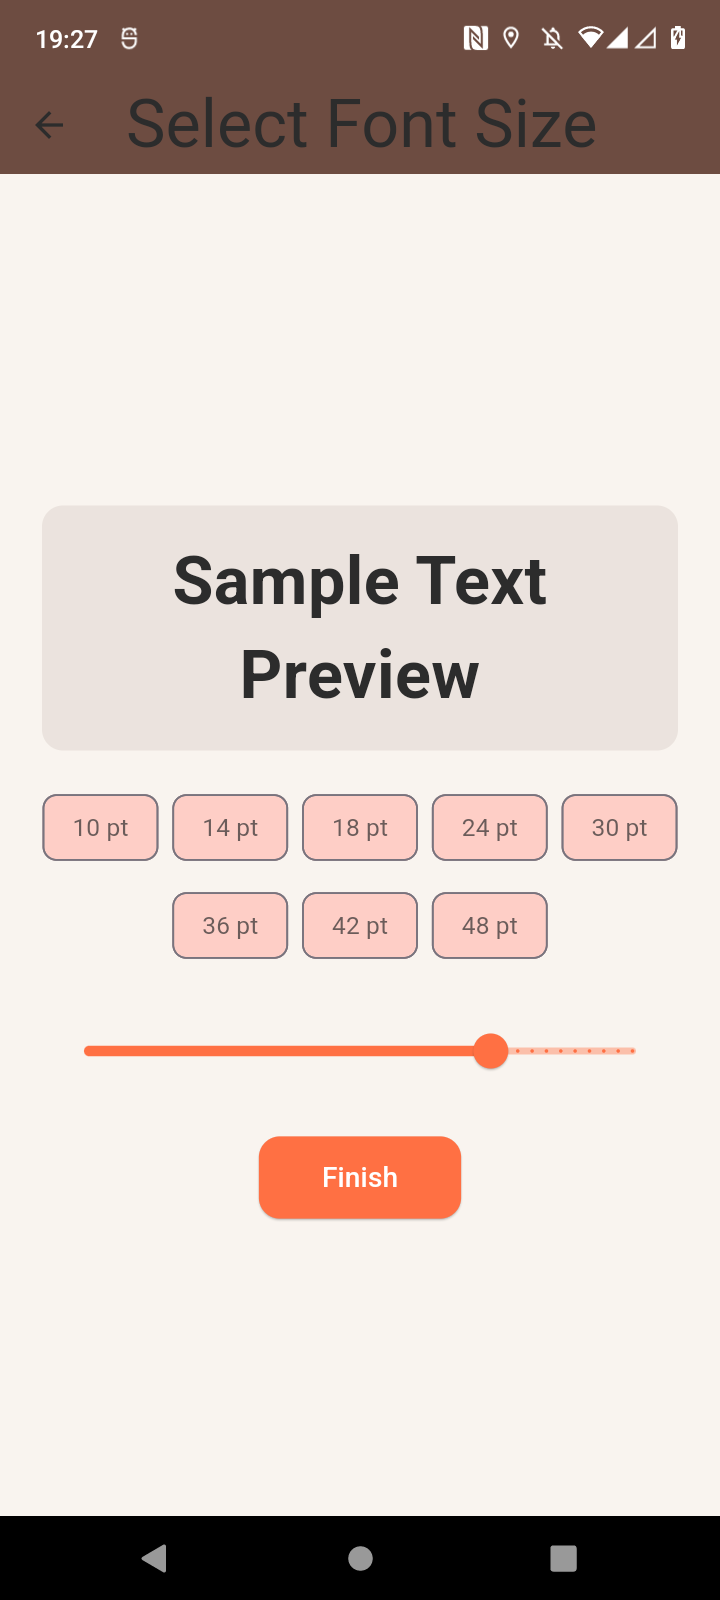
\includegraphics[width=20em]{fontSize.png}
  \end{minipage}
  \hfill
  \begin{minipage}[t]{0.4\textwidth}
    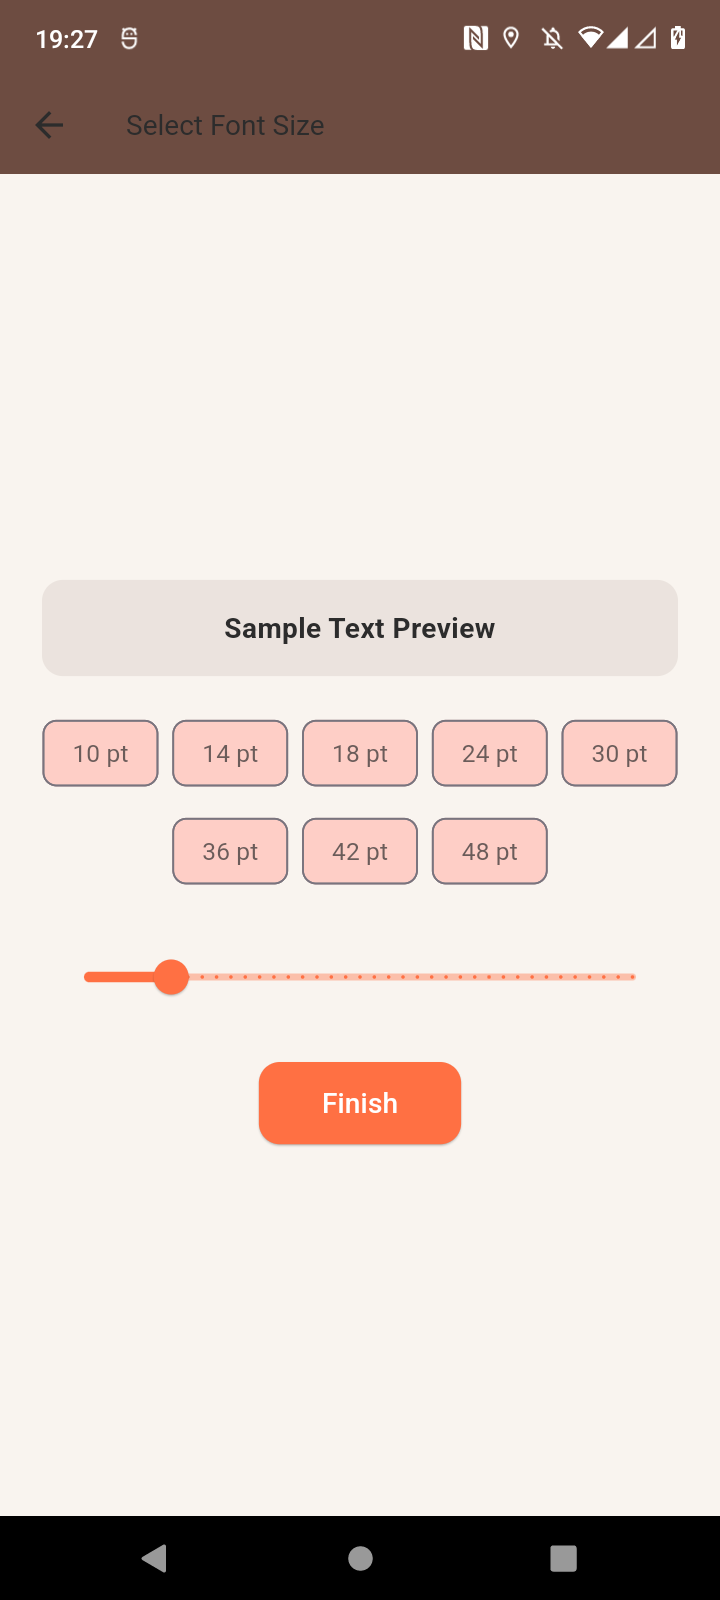
\includegraphics[width=20em]{fontSizeSelection.png}
  \end{minipage}
  \caption{Creme HomePage and recipe page}
  \label{fig:1}
\end{figure*}

\begin{figure*}[ht!]
  \centering
  \begin{minipage}[t]{0.4\textwidth}
    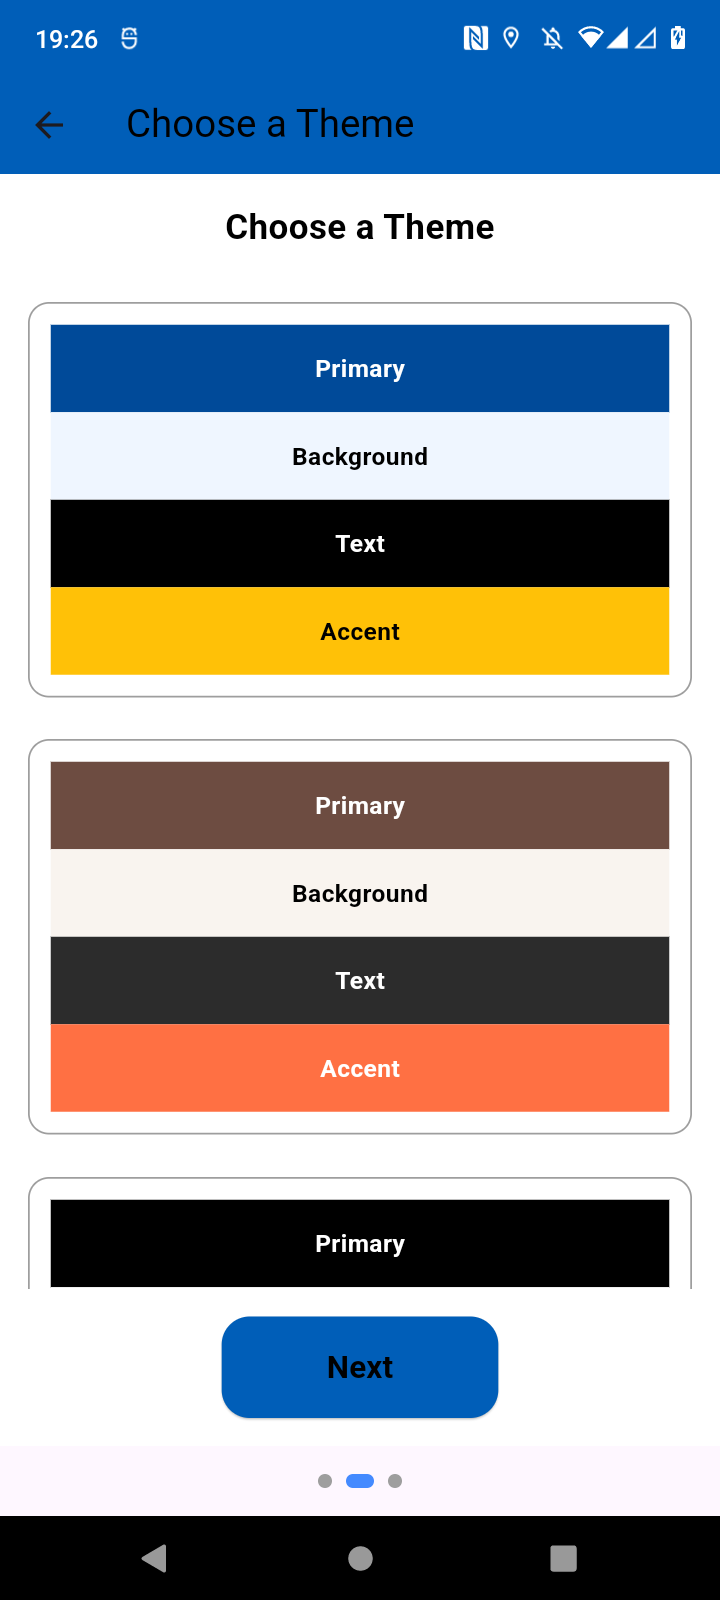
\includegraphics[width=20em]{colourPalette.png}
  \end{minipage}
  \hfill
  \begin{minipage}[t]{0.4\textwidth}
    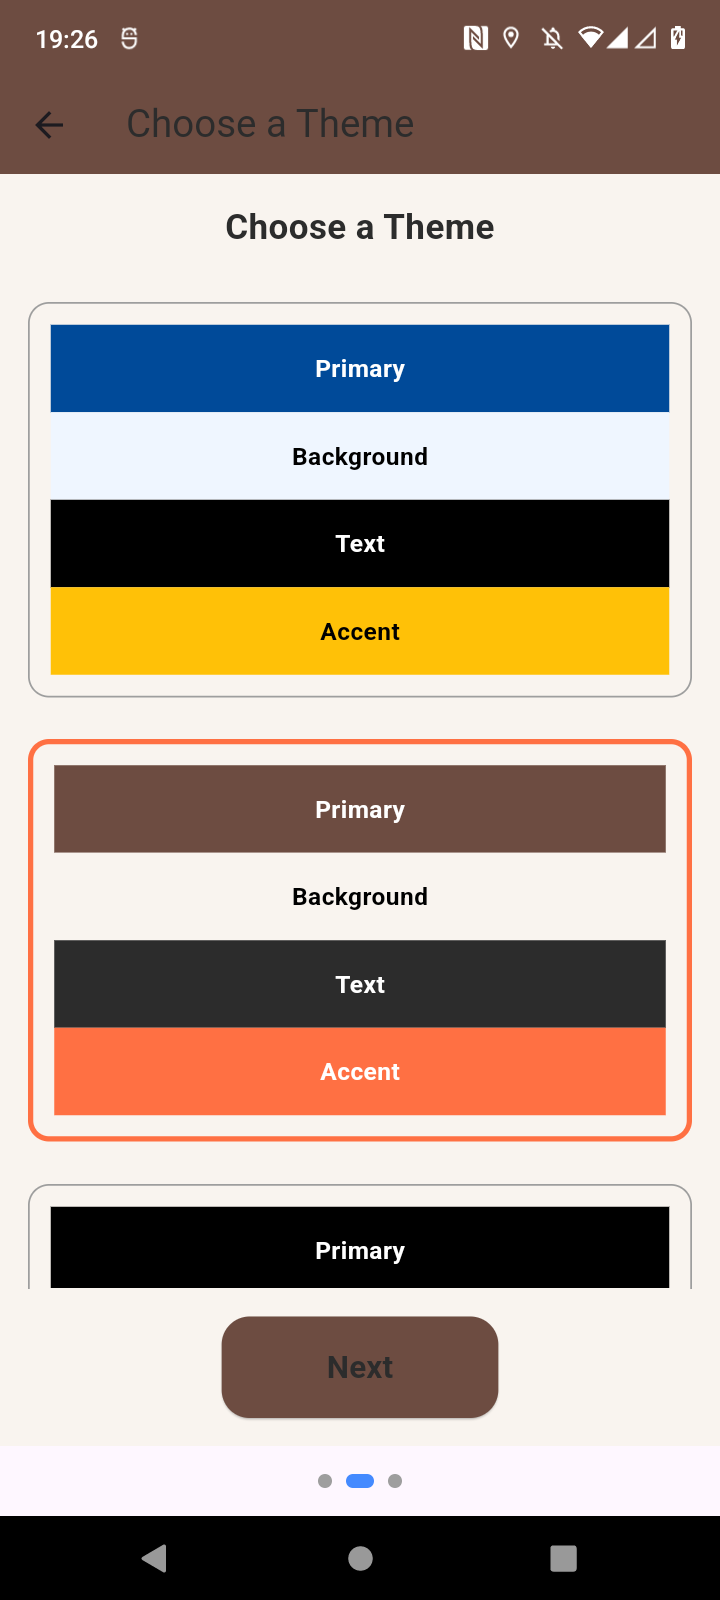
\includegraphics[width=20em]{colourPaletteSelection.png}
  \end{minipage}
  \caption{Creme HomePage and recipe page}
  \label{fig:1}
\end{figure*}

\newpage


Sequential presentation of tasks for cooking reduce intrinsic load and forces the user to focus on one task at a time without being overwhelmed, this is also backed by swellers research which showed the importance of reducing the task complexity.
Simplifyed navigation in the application reduces extraneous load as the user is not required to process of recall a lot of intrstruction at the same time.

The app uses Gestalt principles of similarity to ensiure consistency throughout the application in the forms of button design and colours and shapes to make familiarity for the user throughout the application.
Trappable buttons for next or presious steps for example use size and contrast to guide the users attention throughout the cooking process which was supported by Faradays findings on on visual prominence.

\section{Art Gallery}

The Art Gallery provides a visually engaging platform for showcasing and exploring artwork as well as creating a connection between the user and the artists in collections.Designed to highlight artists collections the interface will use asthetic appeal and intuitive navigation to engage the user.
With the aim of creating a platform which represents the artist and their work effectivitly as well as focusing on the user experience I had to make sure that the artsits where showcases prominently on the main page and the navigation was intuitive, suprising and engaged the used to explore collections that they were attracked to.

\subsection{Relation to HCI}

The grid layout of the Art Gallery used visual hierarchy by changing the sizes of elements dependant on the importance or popularity of the art. It is stated in HCI principles that larger elements on the screen will receive more attention. Therefore larger art pieces will be more popular ones or featured art for example. Smaller pieces will be more obscure or less popular but still visible and clear, this balance or large and small will balance the web page as well as reduce clutter on the page.

The visual hierarchy ensures the users are guided to the most important information first to enhance usability, I will guide them to popular work as this is what the highest percentage of people will enjoy.

\begin{figure*}[ht!]
  \centering
  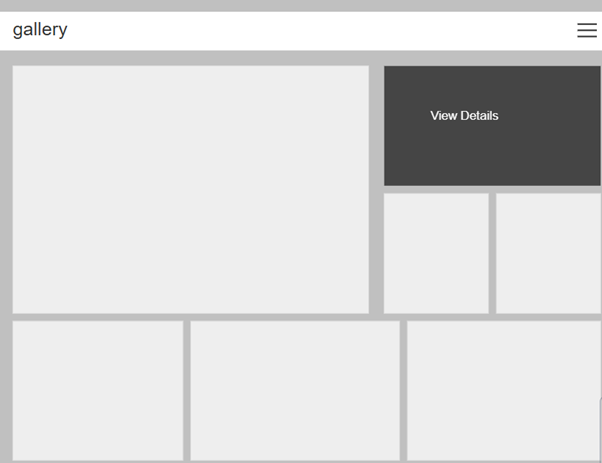
\includegraphics[width=\textwidth]{AG-homepage.png}
  \vspace*{0.0cm}
  \caption{Recipe App Class Diagram}
  \label{fig:1}
\end{figure*}

To reduce cognitive load I have consistently used the same design as well as the same spacing throughout the images. The page will also respond to the user in multiple ways, for example when hovering over an image it will say "view" through text, or the darker colour change and hover animation will visually show the user feedback. This gives the user multiple ways to process information.

\begin{figure*}[ht!]
  \centering
  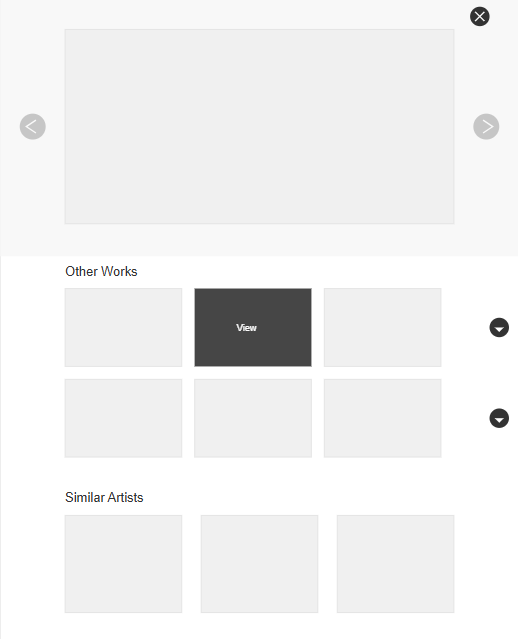
\includegraphics[width=\textwidth]{AG-artist page.png}
  \vspace*{0.0cm}
  \caption{Recipe App Class Diagram}
  \label{fig:1}
\end{figure*}

Accessibility ensures that the website can be used by a variety of different users that face different challenges. The interface is also accessible for the majority of the users as the images act as large clickable areas which makes a simple interaction between the interface and all of the users.


\chapter{Software Engineering}
\section{Diagrams}
\subsection{Travel Planner}

\begin{figure*}[ht!]
  \centering
  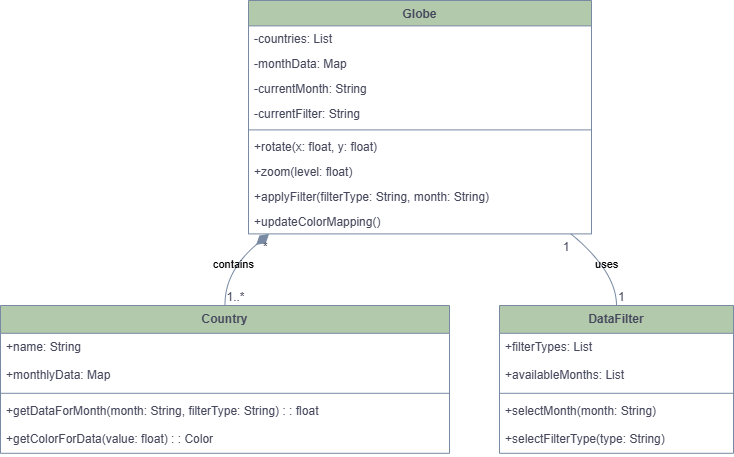
\includegraphics[width=\textwidth]{Travel Planner Class Diagram.png}
  \vspace*{0.0cm}
  \caption{Travel Planner Class Diagram}
  \label{fig:1}
\end{figure*}
\newpage
\begin{figure*}[ht!]
  \centering
  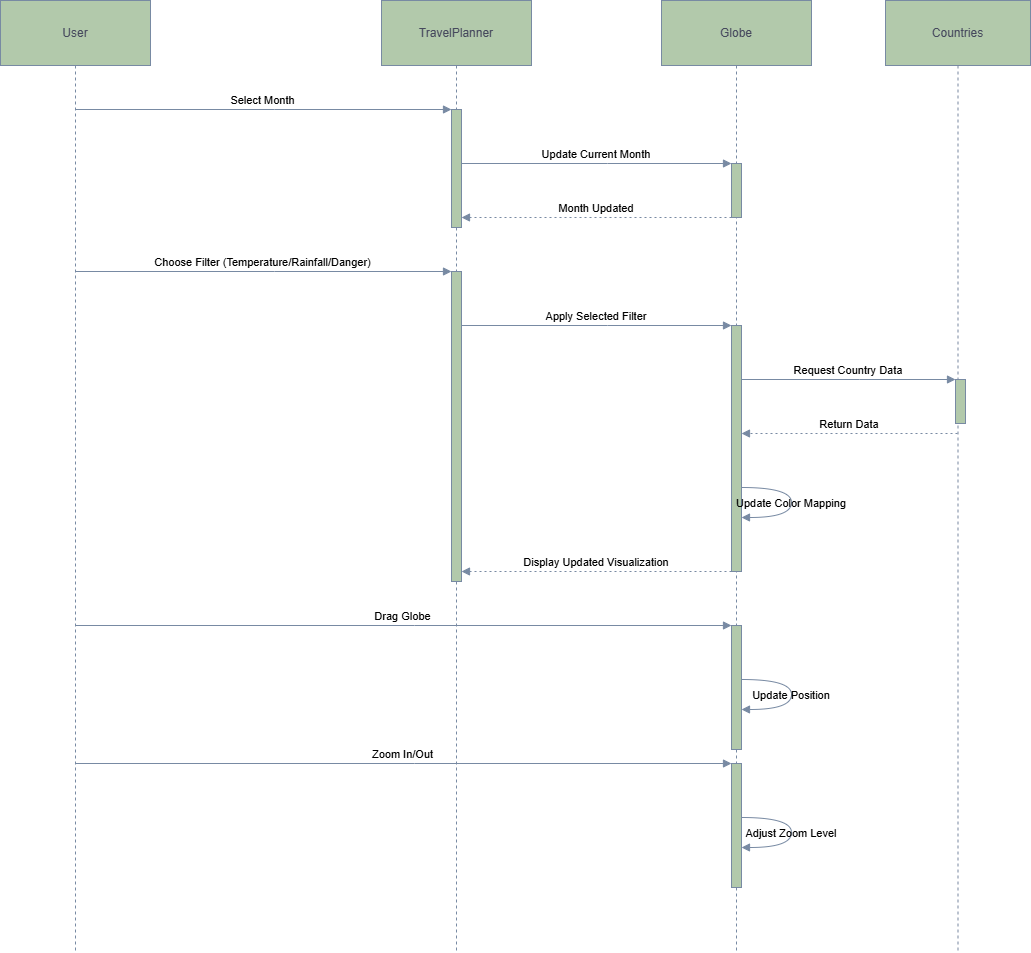
\includegraphics[width=\textwidth]{Travel Planner Sequence Diagram.png}
  \vspace*{0.0cm}
  \caption{Travel Planner Sequence Diagram}
  \label{fig:1}
\end{figure*}


\newpage

\subsection{Recipe App}

\begin{figure*}[ht!]
  \centering
  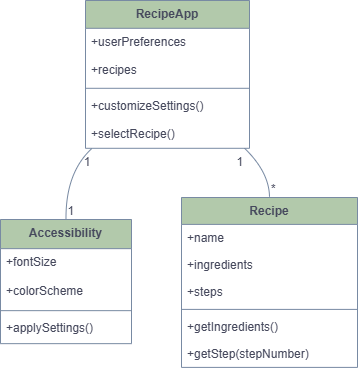
\includegraphics[width=0.6\textwidth]{Recipe App Class Diagram.png}
  \vspace*{0.0cm}
  \caption{Recipe App Class Diagram}
  \label{fig:1}
\end{figure*}
\newpage
\begin{figure*}[ht!]
  \centering
  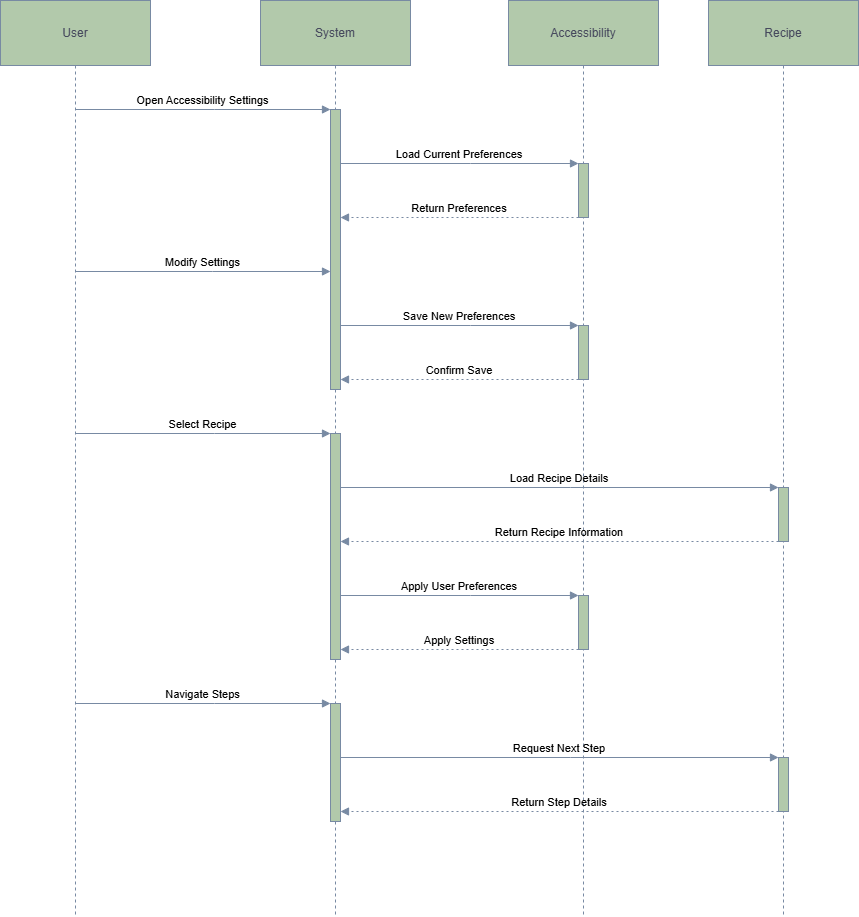
\includegraphics[width=\textwidth]{Recipe App Sequence Diagram.png}
  \vspace*{0.0cm}
  \caption{Recipe App Class Diagram}
  \label{fig:1}
\end{figure*}

\newpage

\subsection{Art Gallery}

\begin{figure*}[ht!]
  \centering
  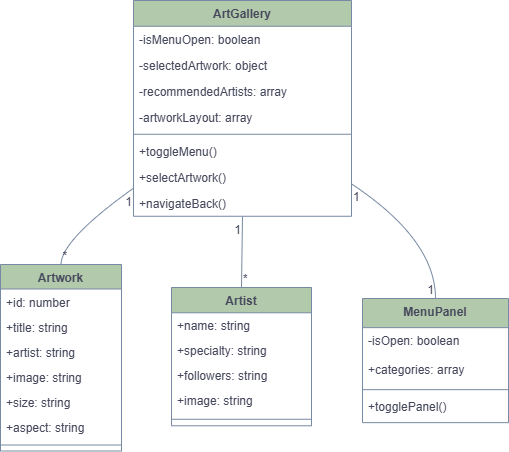
\includegraphics[width=0.8\textwidth]{Art Gallery Class Diagram.png}
  \vspace*{0.0cm}
  \caption{Art Gallery Class Diagram}
  \label{fig:1}
\end{figure*}
\newpage
\begin{figure*}[ht!]
  \centering
  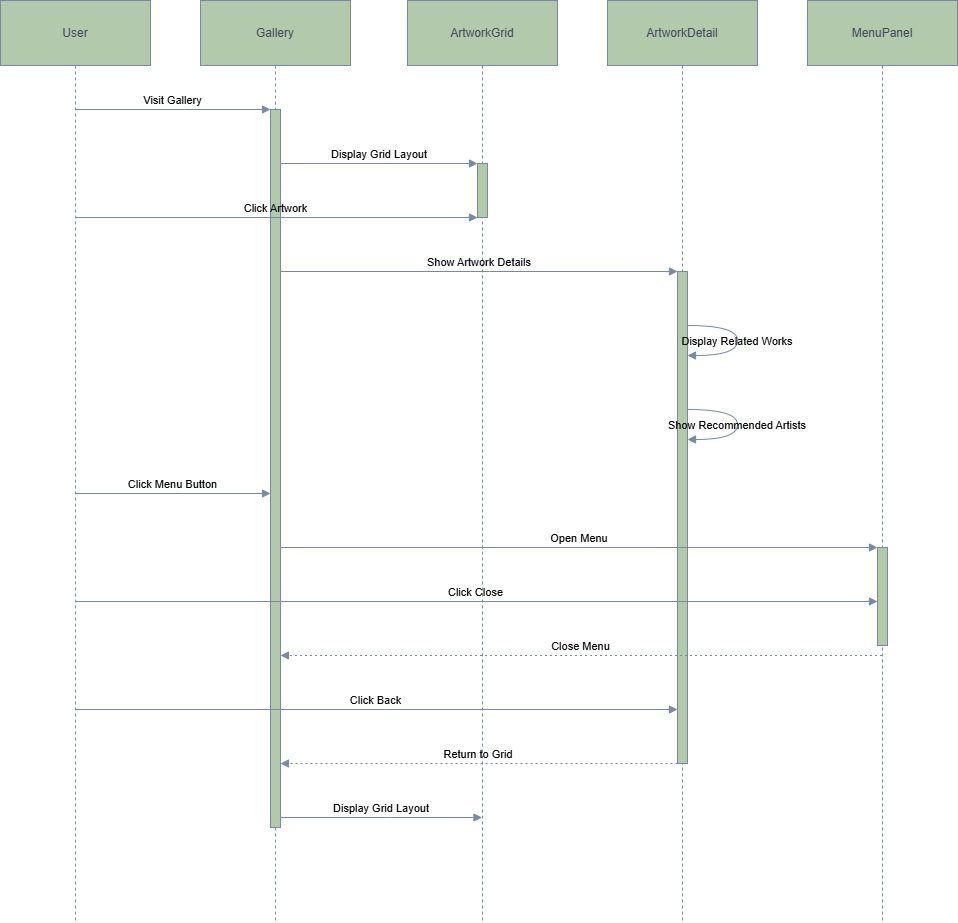
\includegraphics[width=\textwidth]{Art Gallery Sequence Diagram.png}
  \vspace*{0.0cm}
  \caption{Art Gallery Sequence Diagram}
  \label{fig:1}
\end{figure*}



\section{Testing}

Unit Testing has been completed to check functions of the code work, for example the checking if the data is fetched for the filters and month selection when mapping the data in a visual format onto the globe.

Similar tests can be used for components within the Recipe App to test if the functions in the setup are working correctly, ensuring that the font size changes to the users selection and so does the colour palette.

Functional testing has also been complete for the Travel Planner to check if the correct data is displayed. Meaning different colours for filters and that the correct files are fetched and mapped correctly.

\section{Code quality}

Code was organised into reusable components and modules through a modular design which made it eaiser to build and will make it easier to maintain or add componennts in the future.
For example the Travel Planners filters, globe interaction and UI elements were broken into components such as FilterMenu, GolbeRenderer and CountryDetails.
The Recpie app followed the same principles with separate modules for navigation, accessibility settings and recipe steps, although the dart programming language somewhat forces you to implement the required structure.

All of the interfaces had inline comments which are clear and concise for multiple reasons. Firstly the comments explain the logic of some parts of the code which have been researched or where I implemented new techniques or langauges which I am not comfortable with.
Secondly, when further develoeping the code or maintaining it, comments will allow me to scan the code in search of the functions or modules that I am looking for, this makes building on the foundations of the code easier.

\section{Version Control}
Git version control was used throughout the project as it provides many tools to aid development and reduce risks.
Regular commits and pushes to a remote repository ensure that there is another copy of the project and my progress other than locally, this ensure that any local issues such as machine failures would prevent loss of work.

History tracking in git logs every change that was created in the code, therefore previous versions of my code are easy to access in the case that I need to go back.

The most important feature provided is branching, the use of branches means that I am able to develop code, add features and merge to other branches without touching the working code in the main branch. This ensures that there is always working code to present or to go back too.

During the development I stuck to a strict structure within the version control system. Off of the main branch there are 3 branches which act as separate main branches for each interface. This is where the stable and working code is kept. During the setup up of each interface a setup branch was used while a feature branch was used when creating features for the interface. This standard has been used throughout my repository to ensure it is clear which branches contain which information.

\chapter{Appendix}
\section{Diary}

30/09/2024 - Researching papers on HCI issues for project plan

5/10/2024 - Project plan has been completed

15/10/2024 - Have started a seperate diary within in project files, these diaries will contain research and information for developement and will also be the foundation of my report as i am recording all of the information step by step.
Wireframes for Travel Planner have been completed by hand, now i will digitalise them and make them more complex online

20/10/2024 - Completed basic globe implementation through dataset importation.
Will focus on navigation and implemting functions within the navigation

23/10/2024 - Completed month selector with all fucntions working to loading different datasets based on the months.
Next step is to focus on the filters which will load other datasets , and how to implement them by passing the months through the function as well.

27/10/2024 - Attemping to gather all datapoints needed for all of the different filters however some do not exist causing the issue of missing datapoints which i must create based on real data gathered by nations or companies that measure geographical data.

10/11/2024 - Globe complete with seperate diary within the globe branch, now working on the recipe app

11/11/2024 - Research on app production started - what langauges or interfaces to use and how to do it

15/11/2024 - Creation of login page and further research on how to use the dart lanaguage

19/11/2024 - Further developement of login and sign up

24/11/2024 - Research on the colour palletes that should be used and how to present them as well as font sizes

26/11/2024 - Implement the set up page and strucutre of the rest of the app including the main page

28/11/2024 - Going back to find better colour palletes

30/11/2024 - Started gathering information for interim report

04/12/2024 - Started the interim report



\chapter{Videos}
\section{Travel Planner}

https://youtu.be/GRyNZLLVZIQ

\section{Recipe App}

https://youtube.com/shorts/BOfug5pE098?feature=share








%---


\bibliography{interim_refs}
\end{document}
\end{article}